%%%% Better Poster latex template example v1.0 (2019/04/04)
%%%% GNU General Public License v3.0
%%%% Rafael Bailo
%%%% https://github.com/rafaelbailo/betterposter-latex-template
%%%% 
%%%% Original design from Mike Morrison
%%%% https://twitter.com/mikemorrison

\documentclass[a0paper,fleqn]{betterposter}

%%%% Uncomment the following commands to customise the format

%% Setting the width of columns
% Left column
\setlength{\leftbarwidth}{0.25\paperwidth}
% Right column
\setlength{\rightbarwidth}{0.235\paperwidth}

%% Setting the column margins
% Horizontal margin
%\setlength{\columnmarginvertical}{0.05\paperheight}
% Vertical margin
%\setlength{\columnmarginhorizontal}{0.05\paperheight}
% Horizontal margin for the main column
\setlength{\maincolumnmarginvertical}{0.05\paperheight}
% Vertical margin for the main column
%\setlength{\maincolumnmarginhorizontal}{0.15\paperheight}

%% Changing font sizes
% Text font
%\renewcommand{\fontsizestandard}{\fontsize{28}{35} \selectfont}
% Main column font
%\renewcommand{\fontsizemain}{\fontsize{28}{35} \selectfont}
% Title font
\renewcommand{\fontsizetitle}{\fontsize{105}{35} \selectfont}
% Author font
\renewcommand{\fontsizeauthor}{\fontsize{35}{20} \selectfont}
% Section font
%\renewcommand{\fontsizesection}{\fontsize{28}{35} \selectfont}

%% Changing font sizes for a specific text segment
% Place the text inside brackets:
% {\fontsize{28}{35} \selectfont Your text goes here}

%% Changing colours
% Background of side columns
%\renewcommand{\columnbackgroundcolor}{black}
% Font of side columns
%\renewcommand{\columnfontcolor}{gray}
% Background of main column
%\renewcommand{\maincolumnbackgroundcolor}{empirical}
%\renewcommand{\maincolumnbackgroundcolor}{theory}
%\renewcommand{\maincolumnbackgroundcolor}{methods}
%\renewcommand{\maincolumnbackgroundcolor}{intervention}
% Font of main column
%\renewcommand{\maincolumnfontcolor}{gray}

\usepackage{setspace}

\begin{document}


\betterposter{
%%%%%%%% MAIN COLUMN

\maincolumn{
%%%% Main space
\vspace{100pt}

\begin{spacing}{3.5}
    \begin{flushleft}
    {\fontsize{140}{400}\selectfont \textbf{O waste! o waste,}},
    \end{flushleft}
    \vspace{50pt}
    \begin{flushright}
        {\fontsize{140}{10}\selectfont \textbf{wherefore art thou?}}
    \end{flushright}
\end{spacing}

\vspace{340pt}
\begin{minipage}{0.60\textwidth}
    \begin{spacing}{3}
    \begin{center}
            {\fontsize{90}{90}\selectfont \ \textit{With code our guide,}}
        \vspace{40pt}\\
        {\fontsize{90}{90}\selectfont \ \textit{we seek to find,}}
        \vspace{40pt}\\
        {\fontsize{90}{35}\selectfont \textit{hidden hotspots,}}
        \vspace{40pt}\\
        {\fontsize{90}{35}\selectfont \textit{where waste entwined.}}
    \end{spacing}
    \end{center}
\vspace{270pt}
\begin{center}
\begin{spacing}{3}
{\fontsize{46}{40}\selectfont We created the WasteFootprint tool}\\
{\fontsize{46}{40}\selectfont to track supply-chain waste in LCA}\\
\vspace{60pt}
{\fontsize{36}{40}\selectfont View the WasteFootprint code}\\
{\fontsize{36}{40}\selectfont  in our GitHub repository}
\end{spacing}
\vspace{220pt}

\includegraphics[width=0.35\textwidth]{img/qr.svg.eps}
\end{center}
\end{minipage}
\begin{minipage}{0.4\textwidth}
\begin{flushleft}
\vspace{pt}

\includegraphics[width=\textwidth]{img/foot.pdf}
\end{flushleft}
\end{minipage}
%%%% Bottom space
%% This fills the space between the content and the logo
%% QR code
%% Institution logo
\vspace{50pt}


\includegraphics[height=0.1\textwidth]{img/logoUL_white}\hfill

\includegraphics[height=0.07\textwidth]{img/python}\hfill

\includegraphics[height=0.07\textwidth]{img/brightway}\hfill
}

}{
%%%%%%%% LEFT COLUMN

\title{WasteFootprint}
{\fontsizesection\selectfont\textbf{a flexible tool for analysing\\ supply-chain waste flows in LCA}}\\

\vspace{10pt}
\author{Elizabeth Lanphere, Stewart Charles McDowall, Stefano Cucurachi \& Carlos Filipe Blanco Rocha}
\vspace{30pt}
\institution{CML, Leiden University, The Netherlands}

\section{Why?}
\begin{itemize}
    \item To promote `circularity' we must understand waste  
    \item Waste can be a major environmental problem
    \item Most focus on downstream waste (EoL)
    \item Supply-chain waste not well understood
\end{itemize}\\

\section{What?}
\begin{itemize}
\item An extension to the brightway2 LCA framework
\item Calculates waste footprint of a product or service
\item Finds upstream waste flows in a supply chain
\item Categorises waste flows into 14 types
\item Finds hotspots in waste generation
\item Can also do the same for any other flows! \\(e.g., gas, water, critical materials)
\end{itemize}\\

\section{How?}
\begin{itemize}
    \item Explodes database, identifies upstream waste
    \item Exchanges edited and custom methods written
    \item Waste flows become pseudo-biosphere flows
    \item Waste footprint calculated as an LCIA method
\end{itemize}\\

\section{What are the challenges?}
\begin{itemize}
    \item Data completeness: 95\% of waste has no EoL
    \item Waste is not all the same: Sometimes `inert-waste' is just moving some rocks around
    \item LCA system models: both attributional and consequential models make a mess of this
\end{itemize}\\

\section{What next?}
\begin{itemize}
    \item Extension with case studies
    \item Refinement of the method
    \item Application to other flows \\
    (e.g., water, gas, critical materials)
\end{itemize}

}{
%%%%%%%% RIGHT COLUMN
{\fontsizesection\selectfont\textbf{Step by step through the code}}\\

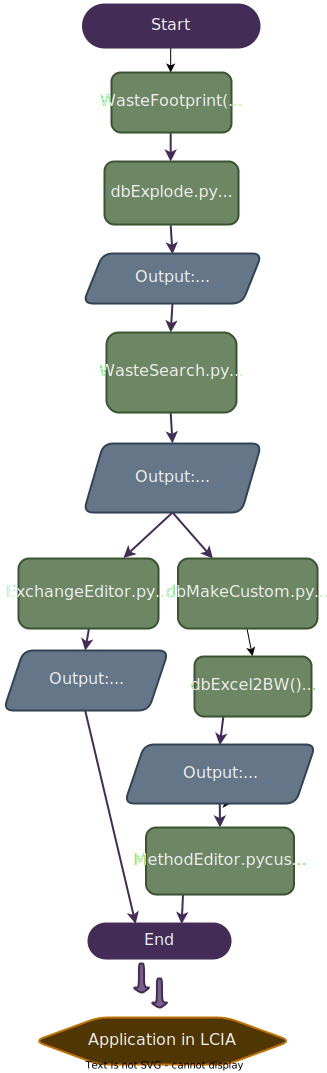
\includegraphics[width=\textwidth]{img/Flowchart_WasteFootprint}

}
\end{document}
